\documentclass[tikz,border=10pt]{standalone}
% Shared look for every TikZ diagram. Load with \input{../../tools/tikz-style.tex}
\usepackage[T1]{fontenc}
\usepackage{lmodern}
\renewcommand{\sfdefault}{lmr}  % diagrams use the same serif as the text
\usetikzlibrary{arrows.meta, positioning, shapes.geometric, calc, fit, backgrounds}
\definecolor{cblue}{HTML}{4C78A8}
\definecolor{corange}{HTML}{F58518}
\definecolor{cgreen}{HTML}{54A24B}
\definecolor{cred}{HTML}{E45756}
\definecolor{cpurple}{HTML}{B279A2}
\definecolor{cgrey}{HTML}{6B6B6B}
\tikzset{
  every picture/.style={font=\sffamily, line width=1.2pt},
  box/.style={draw=#1, fill=#1!12, rounded corners=4pt, align=center, inner sep=7pt, minimum height=1.1cm},
  box/.default=cgrey,
  arrow/.style={-{Stealth[length=3mm]}, draw=cgrey, line width=1.4pt},
  title/.style={font=\sffamily\bfseries\Large},
  note/.style={font=\sffamily\small, text=cgrey, align=center},
}
\AtBeginDocument{\hyphenpenalty=10000 \exhyphenpenalty=10000}

\begin{document}
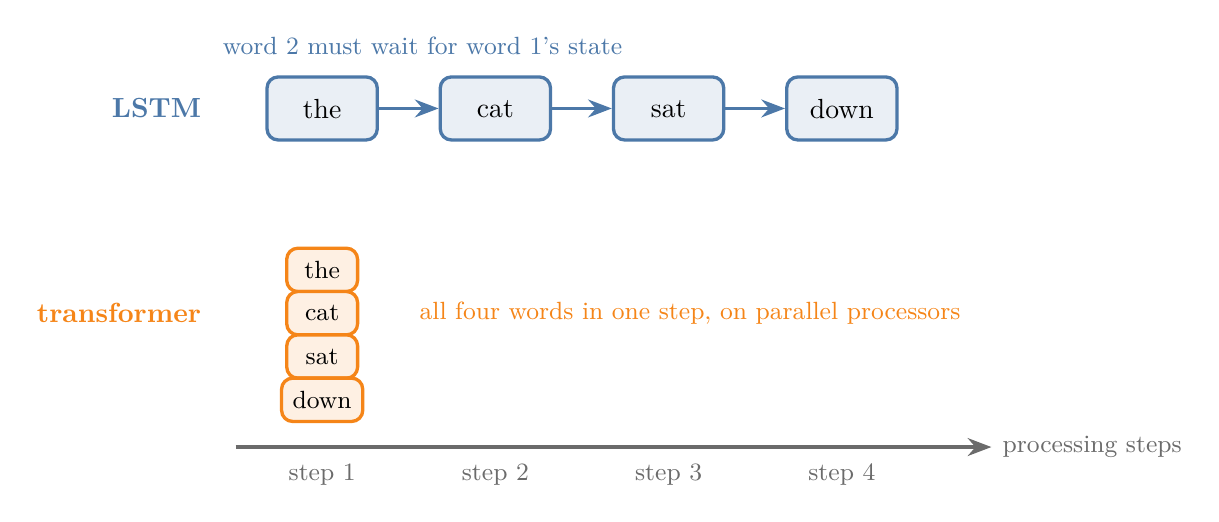
\begin{tikzpicture}[w/.style={box=#1, inner sep=4pt, minimum height=0.8cm, minimum width=1.4cm, font=\sffamily}]
  \draw[arrow] (0,-0.7) -- (9.6,-0.7) node[right, note] {processing steps};
  \foreach \k in {1,...,4} \node[note] at (2.2*\k-1.1,-1.05) {step \k};
  % LSTM
  \node[anchor=east, font=\sffamily\bfseries, text=cblue] at (-0.3,3.6) {LSTM};
  \foreach \w [count=\k] in {the, cat, sat, down} \node[w=cblue] (l\k) at (2.2*\k-1.1,3.6) {\w};
  \foreach \a/\b in {1/2, 2/3, 3/4} \draw[arrow, draw=cblue] (l\a) -- (l\b);
  \node[note, text=cblue, anchor=west] at (-0.3,4.4) {word 2 must wait for word 1's state};
  % transformer
  \node[anchor=east, font=\sffamily\bfseries, text=corange] at (-0.3,1.0) {transformer};
  \foreach \w [count=\k] in {the, cat, sat, down} \node[w=corange, minimum width=0.9cm, minimum height=0.55cm, font=\sffamily\small] at (1.1,2.1-0.55*\k) {\w};
  \node[note, text=corange, anchor=west] at (2.2,1.0) {all four words in one step, on parallel processors};
\end{tikzpicture}
\end{document}
